
\chapter{Aufbau}\label{chap:composition}

Im Rahmen dieses Praktikums soll der Entwurf eines �bertragungssystems von der grundlegenden Idee bis hin zur fertigen Hardware-Implementierung erarbeitet werden. Am Ende steht eine �bertragungsstrecke, die einen einfachen Bitstrom �ber einen Lautsprecher im h�rbaren Bereich �bertr�gt. Die Signale sollen �ber ein Mikrofon aufgenommen und von der nachfolgenden Schaltung demoduliert werden. Sie werden die Strecke zu gro�en Teilen mit dem Simulationstool Matlab beschreiben und simulieren. Nach erfolgreicher Simulation werden sie das beschriebene Modell in geeigneter Weise in Hardware auf einem FPGA umsetzen, um die tats�chliche Funktion zu validieren.
 Um das Praktikum abwechslungsreicher zu gestalten wurde vom gewohnten Ablauf

\begin{itemize}
 	\item Simulation
 	\item Verifizierung
	\item Implementierung auf der Zielhardware
\end{itemize}

des Systementwurfs abgewichen und alle drei Entwurfs-Schritte zusammenh�ngend f�r jedes Modul einzeln durchgef�hrt. 

%
%
%
\chapter{Konventionen}\label{chap:conventions}
\thispagestyle{empty}
%
%
%

\section{Vorbereitung}\label{sec:preparation}

 Als Grundlage f�r dieses Praktikum dient die Vorlesung ``Architekturen der digitalen Signalverarbeitung''. Allerdings ist es nicht zwingend notwendig diese besucht zu haben, da der zur erfolgreichen Durchf�hrung des Praktikums notwendige Stoff in den jeweiligen Grundlagenkapiteln der einzelnen Versuche noch einmal aufgearbeitet wird. Sie sollten aber in jedem Fall die entsprechenden Kapitel vor Beginn des Praktikums aufmerksam durcharbeiten, damit sie die eigentliche Versuchszeit zur Realisierung nutzen k�nnen. 

Sollten sie bisher noch keinen Kontakt mit MATLAB gehabt haben, sollten sie das MATLAB-Tutorial im Anhang \ref{chap:tutorial:matlab} durcharbeiten.

\section{Warnungen und Hinweise}\label{sec:warningsadvices}

Warnungen und Hinweise werden im Skript hervorgehoben.

\prohibit{\textbf{Warnungen} Hier besteht Gefahr, etwas zu besch�digen oder sich zu verletzen.}

\advise{\textbf{Hinweise} Hier wird auf Fehlerm�glichkeiten hingewiesen}

%
%
%
\chapter{Zur Struktur}\label{chap:structure}
\thispagestyle{empty}
%
%
%

Das Skript beinhaltet neben der Praktikumsanleitung ein MATLAB-Tutorium im Anhang \ref{chap:tutorial:matlab} und folgt in der Regel der nachstehenden Struktur.

\begin{enumerate}
	\item Vor�berlegungen
		\begin{itemize}
			\item Konzepte
			\item Realisierungsm�glichkeiten finden
			\item Auswahl einer geeigneten Variante
			\item Gliederung in Teilprobleme
		\end{itemize}
	\item MATLAB
		\begin{itemize}
			\item Programmierung der Module
			\item Aufbau des Modells/der Simulation
			\item Simulation des Entwurfs
		\end{itemize}
	\item VHDL
		\begin{itemize}
			\item Verhaltensmodelle der Module entwerfen
			\item Simulation der einzelnen Module
			\item Simulation des Gesamtentwurfs
			\item Beschreibung der Hardware (RTL)
			\item Simulation des RTL Entwurfs
			\item Implementierung in Hardware
			\item Praxistest und Fehlersuche
			\item Versuchsdurchf�hrung
		\end{itemize}
\end{enumerate}

Gegen Mitte des Praktikums wurde der MATLAB-Teil zusammengefasst und die Struktur nur f�r VHDL beibehalten. Die theoretische Simulation steht am Anfang und kann komplett vollzogen werden. Bei VHDL ist es wichtig, die einzelnen Module getrennt zu verifizieren, da die fehlerfreie Funktion erheblich schwieriger am Gesamtsystem nachzuweisen ist. 

%
%
%
\chapter{Die Hardware}\label{chap:Hardware}
\thispagestyle{empty}
%
%
%

\section{Kurzbeschreibung}\label{sec:HWdesc}


Beim SPATES\footnote{\textbf{SPATES} abk. Signal Processing And Transmission Experiments System} handelt es sich um ein Entwicklungssystem f�r FPGAs der Serie ECP\cite{dsecp} von Lattice. Weiterhin befinden sich noch Komponenten auf der Leiterplatte, die einerseits f�r die Funktion des FPGA (Schaltregler f�r die verschiedenen Versorgungsspannungen, Taktversorgung, usw.), andererseits f�r die Versuche (AD-, DA-Wandler, Mikrofonverst�rker, usw.) notwendig sind.


\section{Vorbereitung der Hardware}\label{sec:HWprep}


Das SPATES besitzt nur relativ wenige Anschlussm�glichkeiten (vgl. Abb. \ref{fig:ADS-Praktikum Leiterplatte} \ifthenelse{\printcolor}{gelb hinterlegt.}{grau hinterlegt.})

\begin{figure} [ht]
	\centering
		\ifthenelse{\printcolor}%
			{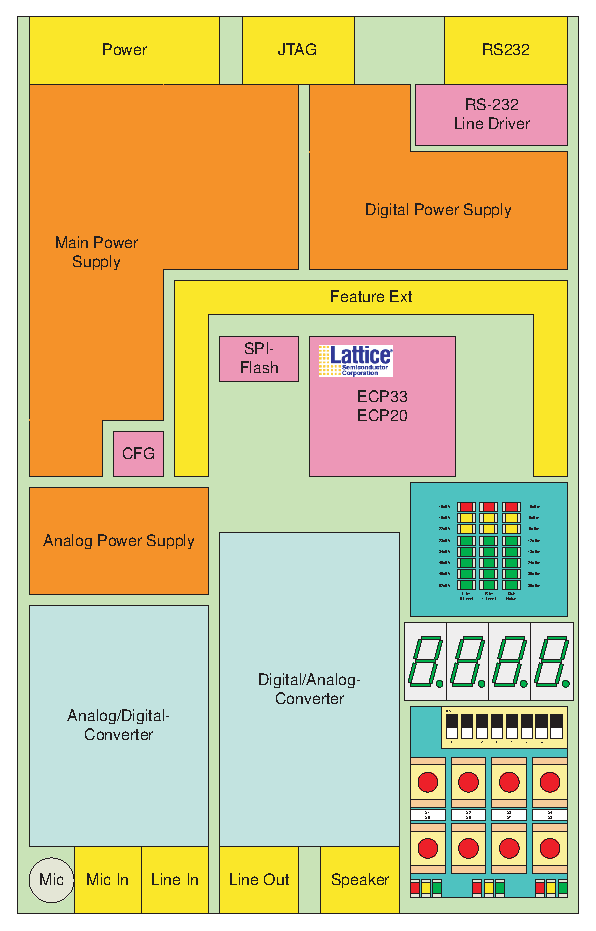
\includegraphics[scale=0.80]{Einfuehrung/bilder/ADS-Praktikum_Leiterplatte.eps}}%
			{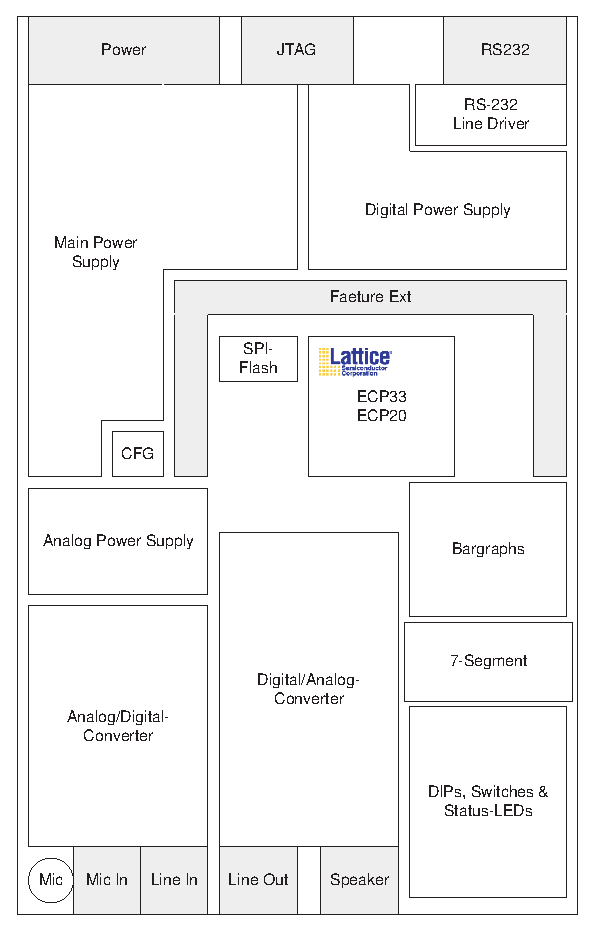
\includegraphics[scale=0.80]{Einfuehrung/bilder/ADS-Praktikum_Leiterplatte_BW.eps}}
	\caption{ADSP-SPATES}
	\label{fig:ADS-Praktikum Leiterplatte}
\end{figure}

\pargraphbox{bilder/global/esd.eps} {Bei der Handhabung ist Vorsicht geboten. Es handelt sich fast ausschlie�lich um Bauteile in	CMOS Technologie.	Zwar besitzen die Schaltkreise inzwischen sehr gute ESD-Schutzschaltungen, dennoch k�nnen diese durch unsachgem��e Handhabung zerst�rt werden. Da die Bauteile teuer sind,	bitte vorher das PC-Geh�use anfassen und sich entladen. Dann sollte nichts passieren.}

Zuerst schalten sie Ihr Netzger�t ein und stellen beide Spannungen auf 15V. Wieder ausmachen und eine Br�cke wie in Abb. \ref{fig:power-short} einstecken, so dass 30V Versorgungsspannung anliegen. Mit dem Adapterkabel (vgl. Abb. \ref{fig:power-cable}) verbinden sie das Netzger�t mit dem SPATES. Der Stecker geht manchmal etwas schwerer, allerdings sollte man keine Gewalt oder ein Messer anwenden m�ssen.


\begin{figure}[ht]
	\centering
	\begin{minipage}[b]{.4\linewidth}
		\centering
		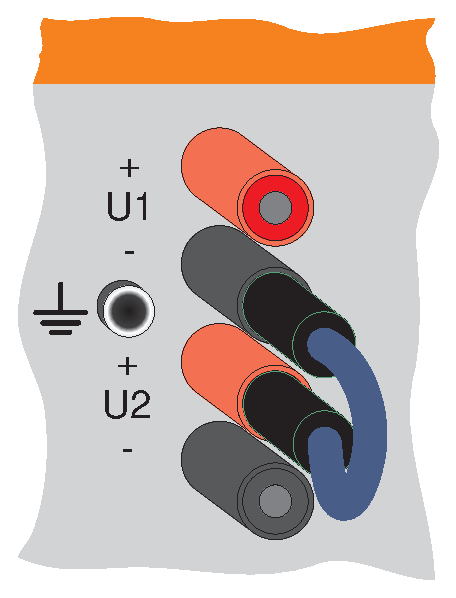
\includegraphics[height=20ex]{Einfuehrung/bilder/power_short.eps}
		\caption{Netzteil-Br�cke}
		\label{fig:power-short}
	\end{minipage}
	\begin{minipage}[b]{.4\linewidth}
	  \centering
		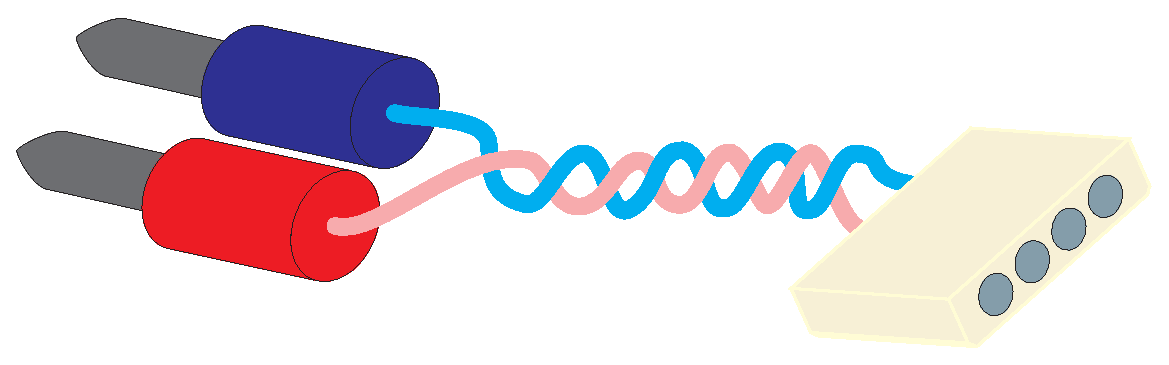
\includegraphics[height=10ex]{Einfuehrung/bilder/power_cable.eps}
		\caption{Power cable}
		\label{fig:power-cable}
	\end{minipage}
\end{figure}

Anschlie�end k�nnen sie das Netzteil wieder einschalten. Zuerst sollten ihnen die verschiedenen Versorgungsspannungs-LEDs auffallen, die eine Funktion der einzelnen Spannungsebenen signalisieren (oder eben auch nicht, dann beim Betreuer melden). Nach einem kurzen Bootvorgang, der durch 2 LEDs direkt neben dem FPGA signalisiert wird, startet auch schon das Diagnose-Programm. Hierbei werden alle LEDs, die 7-Segment-Anzeigen und die Bargraphs kurz angesteuert. Falls der Lautsprecher schon angeschlossen ist, m�sste danach ein kurzer Sweep\footnote{Durchfahren eines Frequenzbereichs z.B. 20Hz bis 20kHz} zu h�ren sein. Ist dieser Test abgeschlossen, so kann man interaktiv alle weiteren Bedienelemente testen. Dabei gilt die Zuordnung aus Tabelle \ref{tab:s2led-assignment}.

\begin{table}
	\centering
	\begin{tabular}{|c|c|}\hline
		\textbf{Schalter/Taster} & \textbf{Anzeigeelement}\\\hline
		S1 & Alle Segmente LD1 \\\hline
		S2 & Alle Segmente LD2 \\\hline
		S3 & Alle Segmente LD3 \\\hline
		S4 & Alle Segmente LD4 \\\hline
		S5 & Alle Segmente Bargraph 1,2 \\\hline
		S6 & Status 1R, 1Y, 1G \\\hline
		S7 & Status 2R, 2Y, 2G \\\hline
		S8 & Status 3R, 3Y, 3G \\\hline
		DIP 1-8 & Bargraph 1,2 LEDs 1-8 \\\hline
	\end{tabular}
	\caption{Zuordnungen der Taster und Schalter}
	\label{tab:s2led-assignment}
\end{table}